
Euler Denklemleri

Üstteki formülü ağdasız / ideal akışkan (inviscid) sıvı için momentum
formüllerini türetmek için kullanacağız. Bu formüllere Euler denklemleri
adı veriliyor. Bu bölümde sıkışmaz (incompressible) akışı göreceğiz.

(3) formülünde momentum dengesi için genel bir ifade var. Euler denklemlerini
elde etmek için gereken (3)'teki eşitliğin en sağındaki kuvvetlerin toplamını
bulmak. Ağdasız akışta ağdalı kaykılma kuvvetlerini (shear forces) yok
sayıyoruz, sıvı öğeleri birbirleri yanından dirençle karşılaşmadan serbestçe
akıyorlar, fakat yerçekimi ve basıncı hala gözönüne almamız lazım.



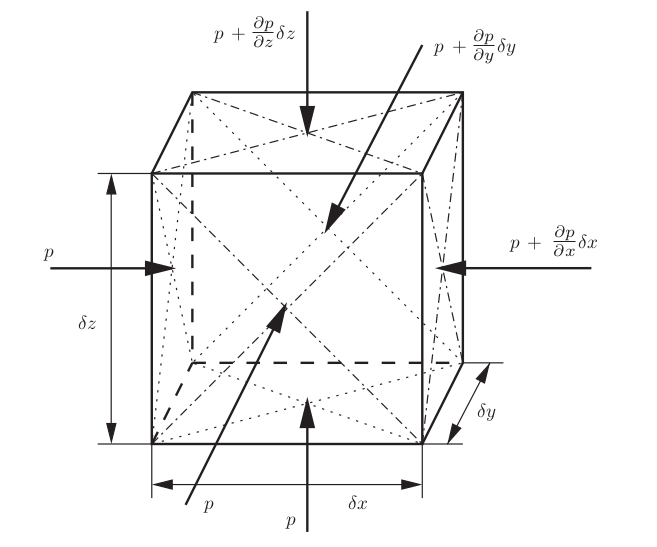
\includegraphics[width=20em]{phy_030_fluid2_05.png}


%%%%%%%%%%%%%%%%%%%%%%%%%%%%%%%%%%%%%%%%%%%%%%%%%%%%%%%%%%%%%%%%%%





Doğu-Batı yönü E,W ile Kuzey-Güney yönü N,S ile Yukarı-Aşağı yönü T,S
ile belirtilecek. 

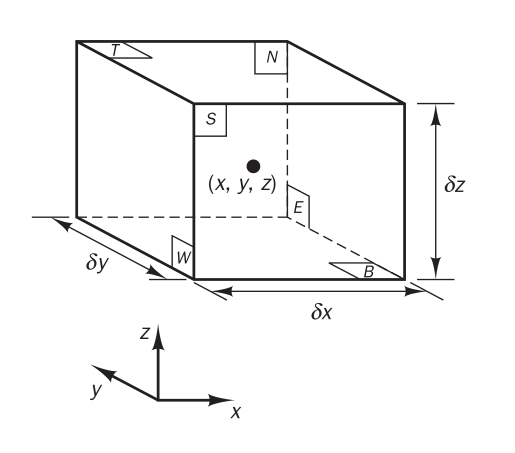
\includegraphics[width=15em]{phy_030_fluid2_03.png}

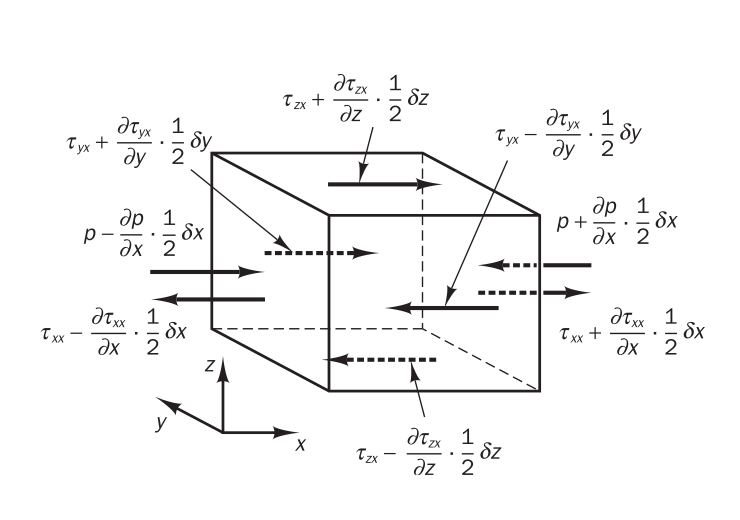
\includegraphics[width=20em]{phy_030_fluid2_01.png}

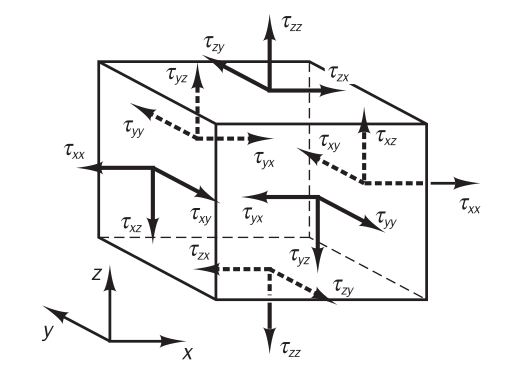
\includegraphics[width=15em]{phy_030_fluid2_02.png}


Ornek olarak $x$ yonundeki kuvvetleri her uc yon icin hesaplayalim.

$E,W$ yüzleri üzerindeki $x$ kuvvetleri, 

$$
\left[
  \left( p - \frac{\partial p}{\partial x} \frac{1}{2} \delta x \right) -
  \left( \tau_{xx} - \frac{\partial \tau_{xx}}{\partial x} \frac{1}{2} \delta x \right) 
\right]
  \delta y \delta z  +
\left[
  -\left( p + \frac{\partial p}{\partial x} \frac{1}{2} \delta x \right) +
  \left( \tau_{xx} + \frac{\partial \tau_{xx}}{\partial x} \frac{1}{2} \delta x \right) 
  \delta y \delta z  +  
\right]
$$

$$
= \left(
-\frac{\partial p}{\partial x} + \frac{\partial \tau_{xx}}{\partial x}
\right)
\delta x \delta y \delta z
$$

$N,S$ yönündekiler,

$$
- \left( \tau_{yx} - \frac{\partial \tau_{yx}}{\partial y}  \frac{1}{2} \delta y
\right) \delta x \delta z  +
\left( \tau_{yx} - \frac{\partial \tau_{yx}}{\partial y}  \frac{1}{2} \delta y
\right) \delta x \delta z  
$$

$$
= \frac{\partial \tau_{yx}}{\partial y} \delta x \delta y \delta z 
$$

$T,B$ üzerindekiler,

$$
- \left(
\tau_{zx} - \frac{\partial \tau_{zx}}{\partial z} \frac{1}{2} \delta z
\right) \delta x \delta y +
\left(
\tau_{zx} + \frac{\partial \tau_{zx}}{\partial z} \frac{1}{2} \delta z
\right) \delta x \delta y 
$$

$$
= \frac{\partial \tau_{zx}}{\partial z} \delta x \delta y \delta z 
$$

Birim hacimdeki üstteki yüzey streslerinin etkisi için üstteki üç sonucu
toplayıp $\delta x \delta y \delta z $ ile böleriz , sonuç,

$$
\frac{\partial (-p + \tau_{xx})}{\delta x} +
\frac{\partial \tau_{yx}}{\partial y} +
\frac{\partial \tau_{zx}}{\partial z} 
$$

